\documentclass[12pt]{article}
\usepackage{geometry}                % See geometry.pdf to learn the layout options. There are lots.
\geometry{letterpaper}                   % ... or a4paper or a5paper or ... 
\usepackage{graphicx}
\usepackage{amssymb}
\usepackage{amsthm}
\usepackage{epstopdf}
\usepackage[english, german]{babel}
\usepackage[utf8]{inputenc}
\usepackage[usenames,dvipsnames]{color}
\usepackage[table]{xcolor}
\usepackage{hyperref}
\DeclareGraphicsRule{.tif}{png}{.png}{`convert #1 `dirname #1`/`basename #1 .tif`.png}
\newcommand{\comment}[1]{}
\usepackage{hyperref}

\theoremstyle{definition}
\newtheorem{example}{Example}

\newenvironment{explanation}{%
   \setlength{\parindent}{0pt}
   \itshape
   \color{blue}
}{}

\newcommand{\projectname}{Dinly}
\newcommand{\productname}{Dinly}
\newcommand{\projectleader}{P. Bauer}
\newcommand{\documentstatus}{In process}
%\newcommand{\documentstatus}{Submitted}
%\newcommand{\documentstatus}{Released}
\newcommand{\version}{V. 1.0}

\begin{document}
\begin{titlepage}
\begin{flushright}

\includegraphics[scale=.5]{htlleondinglogo.png}\\
\end{flushright}

\vspace{10em}

\begin{center}
{\Huge System Specification} \\[3em]
{\LARGE \productname} \\[3em]
\end{center}

\begin{flushleft}
\begin{tabular}{|l|l|}
\hline
Project Name & \projectname \\ \hline
Project Leader & \projectleader \\ \hline
Document state & \documentstatus \\ \hline
Version & \version \\ \hline
\end{tabular}
\end{flushleft}

\end{titlepage}
\section*{Revisions}
\begin{tabular}{|l|l|l|}
\hline
\cellcolor[gray]{0.5}\textcolor{white}{Date} & \cellcolor[gray]{0.5}\textcolor{white}{Author} & \cellcolor[gray]{0.5}\textcolor{white}{Change} \\ \hline
November 03, 2019&P. Bauer&First version \\ \hline
Februar 03, 2020&G. Rechberger&Goal polishing \\ \hline
Februar 03, 2020&J. Richtsfeld& \\ \hline

Februar 03, 2020&M. Hofmarcher&Application domain \\ \hline
\end{tabular}
\pagebreak

\tableofcontents
\pagebreak

\section{Initial Situation and Goal}

\subsection{Initial Situation}
Durch Zeitmangel wird die Ernährung immer schlechter. Diese Aussage wird in folgenden Artikel untermauert: \hyperlink{https://www.gesund.at/ernaehrung/gesunde-ernaehrung-zeit/}{\color{blue}Ist der Zeitmangel wirklich schuld an der schlechten Ernährung?}


Die Bevölkerung möchte tendenziell weniger Zeit für die Planung und Zubereitung von Mahlzeiten aufwenden. Da in der Eile oft, keine Ideen für neue Speisen vorhanden sind, wird die Ernährung schnell eintönig und unausgewogen. Daher greifen viele Leute aufgrund des Zeitmanges auf Fast Food zurück, welches besonders ungesund ist. 

Selbst zu kochen kann hingegen positive Auswirkung auf die physische und mentale Gesundheit haben, wie zum Beispiel dieser Bericht zeigt:
\hyperlink{https://www.huffpost.com/entry/cooking-longevity_n_1518466?guccounter=1&guce_referrer=aHR0cHM6Ly93d3cuZ29vZ2xlLmNvbS8&guce_referrer_sig=AQAAAD3kSnBoydOhZwbnnWL-ifUA6FwaQfkqdJv0bSVaUdyuhl4C6NVEeAAiluGbP9UVwuqUbucdfEpI52AC8rfEJkO3KkpP64ZMdVRKjGck46ZzFhcoiL22O4cm3ARE7xv_Iy1_wFgeMpTcOUYfxZ8hvpvg-gfYQlpe_FKIpiW4nF30}{\color{blue}Bericht zur Cambridge Studie zur Ernährung}.
 Die angespannte Zeitsituation wird noch schwieriger wenn man zusätzlich Sport betreibt und seine Kalorienzufuhr überwachen möchte. Dazu kommt, dass man seine Lebensmitteleinkäufe gut planen muss, um Abfälle zu vermeiden und Geld zu sparen.

\subsection{Application Domain}
Unsere Vision ist, möglichst viele Leute zum Kochen zu bewegen und sie somit auf Dauer zu einem gesünderen Leben zu bewegen. Wir wollen dem Kunden mehr Übersicht über sein Konsumverhalten geben und Bewusstsein für gesunde Ernährung schaffen. Desweiteren wollen wir Nutzer mit Rezepten inspirieren und ihnen das alltägliche ``Was soll ich denn bloß kochen?''        ersparen. Wenn wir dies schaffen, reduzieren wir auch die Chance, dass Leute durch Unkreativität zum FastFood Restaraunt essen gehen. Das optimale Resultat wäre eine Verbesserung der Gesundheit und somit Lebensqualität des Nutzers ohne dabei viel Zeit aufwenden zu müssen. Außerdem können Hobbyköche ihre Künste und Kreationen auf unsere Plattform hochladen und Feedback von anderen Nutzern erhalten. 

Was Konkurrenz betrifft, gibt es eine Applikation namens Yummly, welche bereits 5 Millionen Nutzer im Google Play Store hat. Diese ist in den Staaten bereits sehr etabliert und verfügt über alle Rezepte, welche einem in den Kopf kommen könnten. Wir werden deswegen sehr viel Wert auf unseren Ernährungsplan- generator legen, um ein Alleinstellungsmerkmal zu schaffen. Außerdem werden wir versuchen, unsere Applikation noch mehr an das Kochhobby des Nutzers zu binden und jegliche Möglichkeiten zur Communitybildung zu nutzen.

Ein weiterer Konkurent wäre Chefkoch, sie bieten auch eine Bestellfunktion (jedoch nur in Deutschland) und zeigen die Kalorienzahl einer Mahlzeit an(wir wollen zusätzlich die Makros anzeigen). 

Ein Beispiel hierzu wäre eine ``Teilen`` Funktion, die es dem Nutzer ermöglicht, das Gekochte mit Referenzen auf unsere Applikation in der Story einer seiner Social-Media Platformen zu posten. Dies motiviert Andere, die dann auch dieses Rezept mithilfe unserer Applikation probieren.


\subsubsection{Glossary}
\begin{tabular}{|p{.2\linewidth}|p{.65\linewidth}|}
\hline
Community & Eine Gruppe von Nutzer, die unsere App benutzen und als gemeinsames Ziel verfolgen sich gesünder und ausgewogener zu ernähren. \\
\hline 
Fast Food & In Massenproduktion hergestellte, standardisierte Speisen, die für den schnellen Verzehr gedacht sind und daher meist ungesund.  \\ 
\hline 
Mahlzeit & Essen , das aus verschiedenen kalten oder warmen Speisen zusammengestellt ist und durch unser System vorgschlagen wird.\\ \hline
Kalorienzufuhr & Zufuhr von Energie durch Nahrungsaufnahme   \\ 
\hline 
\end{tabular}


\subsection{Goal}
Unsere Projektziele sind, eine App zu entwickeln mit der sich die Nutzer mit weniger Arbeit und Zeit gesünder und ausgewogener ernähren können. Desweiteren wollen wir eine Community aufbauen wollen, in welcher Nutzer ihren Kocherfolg auf sozialen Medien teilen, um noch mehr Nutzer aufbauen zu können. Auch wollen wir Nutzer inspirieren häufiger selbst zu kochen, um sich daher gesünder und ausgewogener ernähren und seltener auf ungesunde Fertiggerichte oder Fastfood zurückgreifen. Ein weiteres Ziel ist es, dass sich die Nutzer durch die gezielten und durchgeplanten Lebensmitteleinkäufe Geld sparen. Natürlich wird durch diese gezielte Einkäufe auch Lebensmittelabfälle reduziert und daher die Umwelt geschont.
\pagebreak

\section{Functional Requirements}

\subsection{Overview}
\begin{center}
    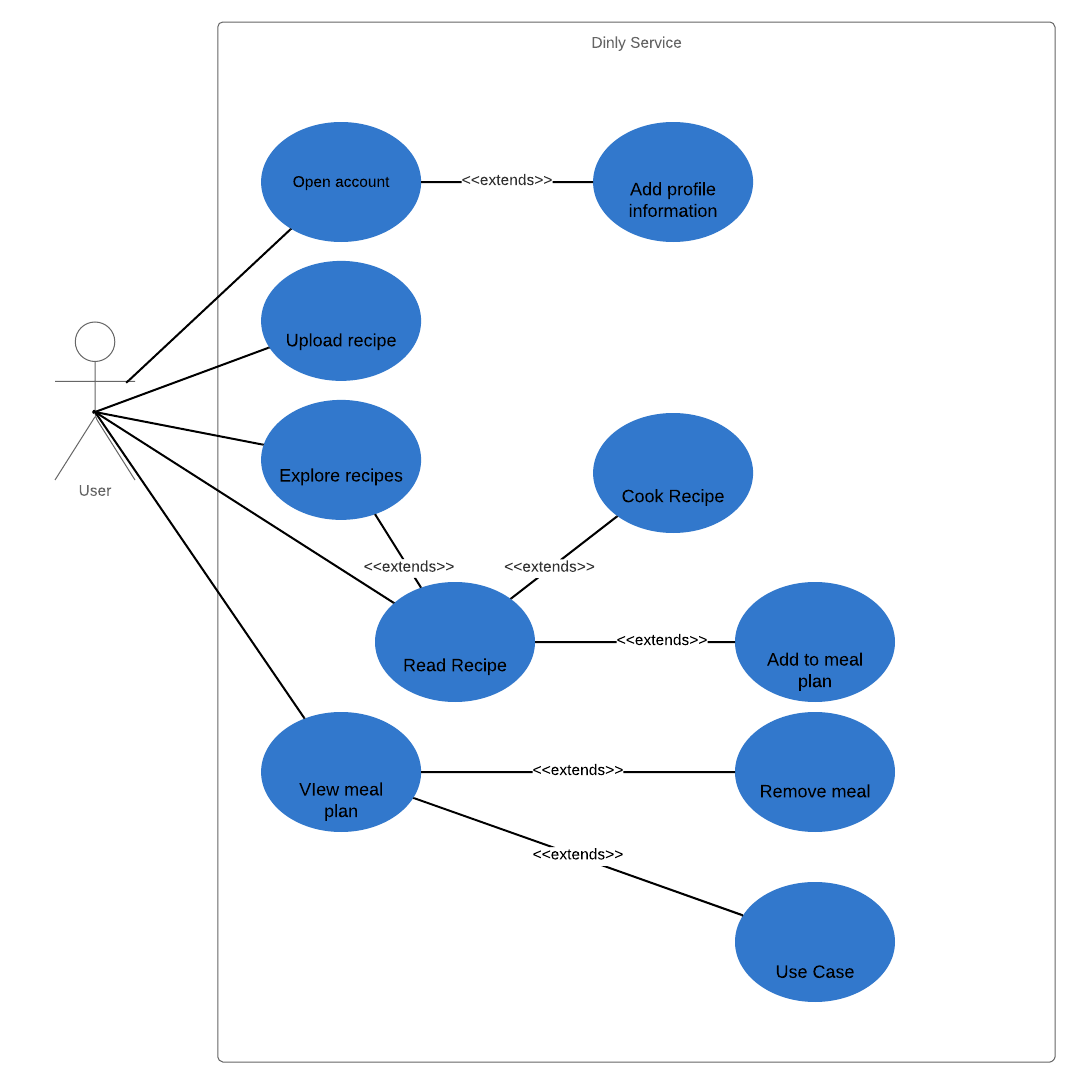
\includegraphics[width=1.1\textwidth]{res/images/UseCaseDiagram.png}
\end{center}

\subsubsection{Mahlzeitenübersicht}
Planung jeweils für eine Woche im Voraus, optionales eintragen der Essenszeiten in den Kalender
Nutzer können Gerichte ändern, weil z.B. zu aufwändig, schmeckt nicht, usw.. Über diese Übersicht kommt man auf die einzelnen Rezepte und kann sich diese näher ansehen.

\subsubsection{Spezifische Auswahl der Mahlzeiten}
Sollte der Nutzer mit den vom System ausgewählten Mahlzeiten aus der Mahlzeitenübersicht nicht zufrieden sein, kann er diese natürlich ändern.
Dazu verwendet er dann die integrierte Rezeptsuche, die auf jeden Nutzer genau zugschnitten ist.

\subsubsection{Rezeptsuche}
Diese Auswahl/Suche von Rezepten und Mahlzeiten basiert auf Rezepten mit denen der Nutzer schon in der Vergangenheit zufrieden war, ähnliche Mahlzeiten/Rezepte werden dann dem Nutzer bevorzugt vorgeschlagen und empfohlen. Diese Vorschläge basieren des Weitern auch auf den Daten bei der Registrierung, um dem Nutzer Rezepte anzubieten die perfekt zum ihm/ihr passen.

Rezepte könne
nach Rezepte müssen natürlich auch Filter wie z.B.: vegan, vegetarisch, Unvertraeglichkeiten, Intoleranzen gesetzt werden können, um dem Nutzer eine gezielte Suche zu erleichtern. 

\subsubsection{Kalorientracker}
Auf einer eigenen Seite können Nutzer ihre konsumierten Kalorien und Makronährstoffe \(Kohlenhydrate, Eiweiße, Fette\) sehen, diese basieren auf den Mahlzeiten aus der Mahlzeitenübersicht.

\subsubsection{Einkaufsliste}
Die für die Zubereitung der Rezepte benötigten Lebensmittel werden in einer Einkaufsliste notiert. Die Nutzer können nun bereits gekaufte Lebensmittel austragen und den Rest direkt über unsere App bestellen und sich nach Hause liefern lassen. Um eine zusätzliche Einkaufsliste zu vermeiden, können auch Artikel die nicht für die Zubereitung der Mahlzeit benötigt werden eingetragen werden. 

Ebenfalls angedacht ist die Reihenfolge der Artikel in der Einkaufsliste an die Reihenfolge in der sie im Supermarkt stehen anzugleichen. Dabei soll vor allem die Gruppierung nach den Kategorien erfolgen, um den Einkauf im Supermarkt zu erleicht und zu beschleunigen.

\subsubsection{Teilen}
Die Nutzer können ihre zubereitete Mahlzeit direkt auf Social Media Platformen wie z.B. Instagram, Facebook teilen. Dies ist wichtig um eine Community rund um unsere App aufzubauen und kostenlos Werbung zu betreiben. Auch entsteht durch diese Funktion eine stärker Bindung zwischen Nutzer und App, da man öffentlich wirbt diese App zu benutzen.

\subsection{Use Case 1: Kalender Slide}
\subsubsection{General Description}
\begin{tabular}{|p{.2\linewidth}|p{.65\linewidth}|}
\hline 
ID: & Calender slide \\ \hline
Goal: & Essensplan für die nächste Woche anzeigen \\ \hline
Precondition: & Klicken des "Essenplans"-Buttons im Menu\\ \hline
Postcondition: & Der Essensplan wurde angezeigt. \\ \hline
Involved Users: &Role name: Benutzer der App \\ \hline
\end{tabular}

\subsubsection{UI to call the use case}


\begin{center}
    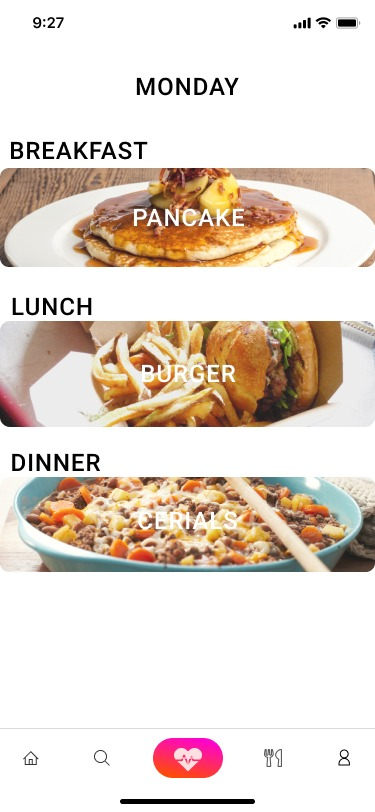
\includegraphics[width=0.4\textwidth]{res/images/Calendar.jpeg}
\end{center}


\subsubsection{The Standard Use}
Der Nutzer klickt auf den Essensplan-Button im Menu. Danach wird ihm/ihr der Plan für die nächste Woche angezeigt.

\subsubsection{The Non-Standard Use}
User hat keine Internetverbindung. Dies führt zu einer sofortigen Fehlermeldung die den User darauf hinweißt, die Verbindung herzustellen 



\pagebreak
\subsection{Use Case 2: Gerichtdetails}
\subsubsection{General Description}

\begin{tabular}{|p{.2\linewidth}|p{.65\linewidth}|}
\hline 
ID: & Specific Selection of the Meal \\ \hline
Goal: & Anzeigen der Mahlzeit mit Inforamtionen \\ \hline
Precondition: & Mahlzeit im Calendar Slide wurde angeklickt \\ \hline
Postcondition: & Mahlzeit und essentielle Informationen wurden angezeigt \\ \hline
Involved Users: &Role name: Benutzer der App \\ \hline
\end{tabular}

\subsubsection{UI to call the use case}

\begin{center}
    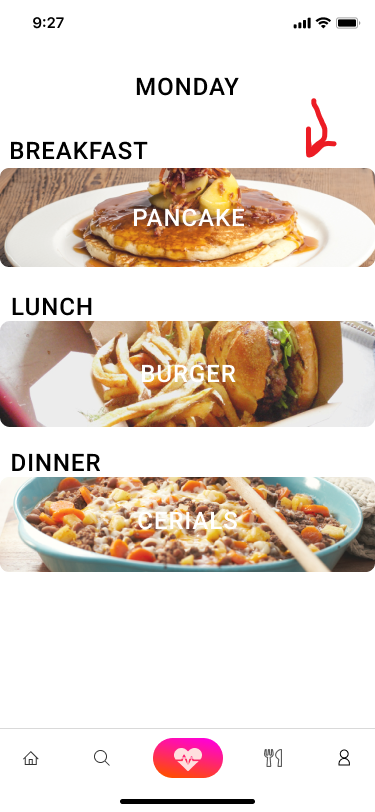
\includegraphics[width=0.35\textwidth]{res/images/MenueClick.png}
\end{center}

Der Nutzer klickt auf den Pancake und kommt hiermit zur Spezifischen übersicht für die Mahlzeit.
\subsubsection{The Standard Use}
\begin{center}
    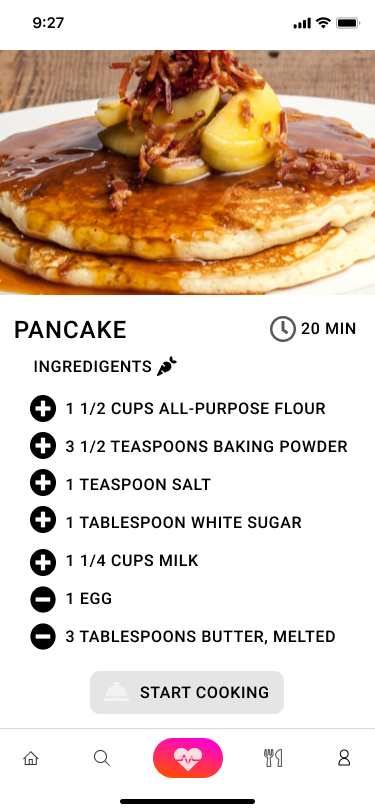
\includegraphics[width=0.5\textwidth]{res/images/Breakfast.png}
\end{center}


Der User kann hier die eine Übersicht über das Gericht erhalten. Darüber hinaus kann man gleich alle benötigten Lebensmittel für die ausgewählte Portion in den Warenkorb hinzufügen. Hier wird auch der User über Nährwerte und die Kochdauer informiert.




\pagebreak

\subsection{Use Case 3: Rezeptsuche}
\subsubsection{General Description}

\begin{tabular}{|p{.2\linewidth}|p{.65\linewidth}|}
\hline 
ID: & ReciptSearch \\ \hline
Goal: & Finden des gesuchten Rezeptes \\ \hline
Precondition: & Wenn der Nutzer auf den Suchen Tab clickt \\ \hline
Postcondition: & Der Nutzer hat sein gesuchtes Rezept gefunden \\ \hline
Involved Users: &Role name: Benutzer der App \\ \hline
\end{tabular}

\subsubsection{UI to call the use case}

\begin{center}
    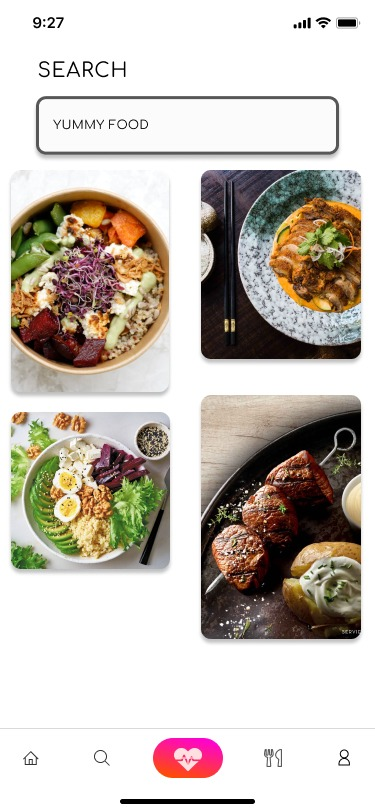
\includegraphics[width=0.4\textwidth]{res/images/Search.jpeg}
\end{center}


\subsubsection{The Standard Use}
Der Nutzer klickt auf Suchen gibt seinen Suchbegriff und evtl Filter ein und findet sein gesuchtes Rezept.


\subsubsection{The Non-Standard Use}
Der Benuter sucht nach einem Rezept welches es nicht gibt. Er bekommt einen leere Seite mit dem Hinweis, dass nichts gefunden wurde.
\pagebreak



\subsection{Use Case 4: Kalorientracker}

\subsubsection{General Description}

\begin{tabular}{|p{.2\linewidth}|p{.65\linewidth}|}
\hline 
ID: & CalorieTracker \\ \hline
Goal: & Der Nutzer bekommt eine Übersicht über alle Nährwerte die er an diesem Tag verzerrt hat.\\ \hline
Precondition: & Wenn der Nutzer auf den Kalorien Tab geht. \\ \hline
Postcondition: & Der Nutzer bekommt seine Nährewerte angezeigt. \\ \hline
Involved Users: &Role name: Benutzer der App \\ \hline
\end{tabular}

\subsubsection{UI to call the use case}

\begin{center}
    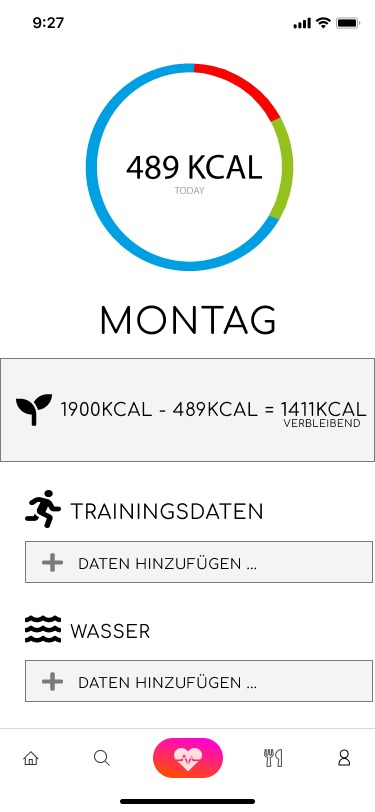
\includegraphics[width=0.4\textwidth]{res/images/CalorieDashboard.jpeg}
\end{center}


\subsubsection{The Standard Use}
Der Nutzer klickt auf den Kalorientracker Tab und bekommt eine Auswertung seiner konsumierten Nährwerte präsentiert. Darüber hinaus kann der User seine tägliche Menge von konsumierten Wasser angeben.

\subsubsection{The Non-Standard Use}
Der Nutzer hat an diesem Tag noch nichts gegessen oder keine Daten eingegeben und somit kann keine Nährwertaufschlüsselung präsentiert werden.
\pagebreak



\subsection{Use Case 5: Einkaufsliste}

\subsubsection{General Description}

\begin{tabular}{|p{.2\linewidth}|p{.65\linewidth}|}
\hline 
ID: & ShoppingList \\ \hline
Goal: & Eine Einkaufsliste mit allen Benötigten Zutaten. \\ \hline
Precondition: & Wenn der Nutzer auf den Einkaufslisten Tab klickt. \\ \hline
Postcondition: & Der Nutzer bekommt eine Liste aller benötigter Zutaten präsentiert. \\ \hline
Involved Users: &Role name: Benutzer der App \\ \hline
\end{tabular}

\subsubsection{UI to call the use case}
\begin{explanation}
\begin{figure}[h!]
    \begin{center}
        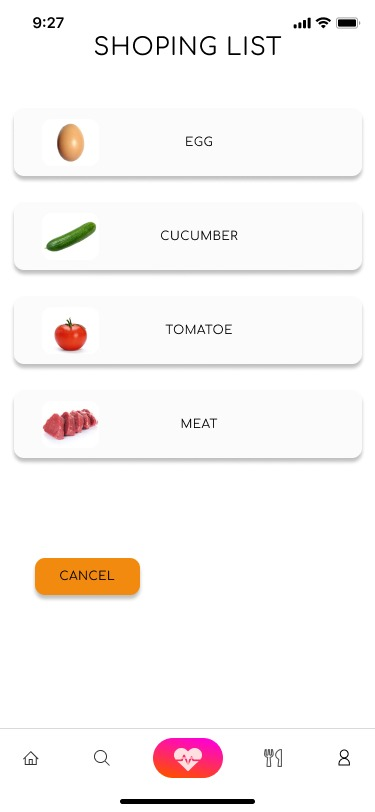
\includegraphics[width=0.5\textwidth]{res/images/ShoppingList.jpeg}
        \caption{Einkaufsliste}
    \end{center}
\end{figure}\end{explanation}

\subsubsection{The Standard Use}
Der Nutzer wählt bei allen Rezepten aus ob er die Zutaten in die Einkaufsliste hinzufügen möchte. Nun kann er auf den Einkaufslisten Tab navigieren und alle benötigten Zutaten direkt bestellen oder manuell austragen falls er manche Zutaten bereits besitzt oder er die Zutaten selbst im Einzelhandel kauft. Zusätzlich kann er einen beliebigen Eintrag erstellen um nicht noch eine zusätzliche Einkaufsliste zu benötigen.

\subsubsection{The Non-Standard Use}
Der Lieferant hat manche Lebensmittel evtl. nicht im Angebot diese müssen hervorgehoben werden und der Nutzer darauf aufmerksam gemacht werden, dass er diese anderweitig beziehen muss. Dies ist besonders relevant wenn der Nutzer eigene Artikel eingetragen hat.
\pagebreak

\subsection{Use Case 6: Teilen}

\subsubsection{General Description}

\begin{tabular}{|p{.2\linewidth}|p{.65\linewidth}|}
\hline 
ID: & Teilen \\ \hline
Goal: & Ein Foto der Zubereiteten Mahlzeit via Socialmedia zu tielen \\ \hline
Precondition: & Beim Fertigstellen einer Mahlzeit \\ \hline
Postcondition: & Ein Bild mit Wasserzeichen wurde auf Socialmedia geteilt\\ \hline
Involved Users: &Role name: Benutzer der ein Rezept zubereitet hat \\ \hline
\end{tabular}

\subsubsection{UI to call the use case}
\begin{center}
    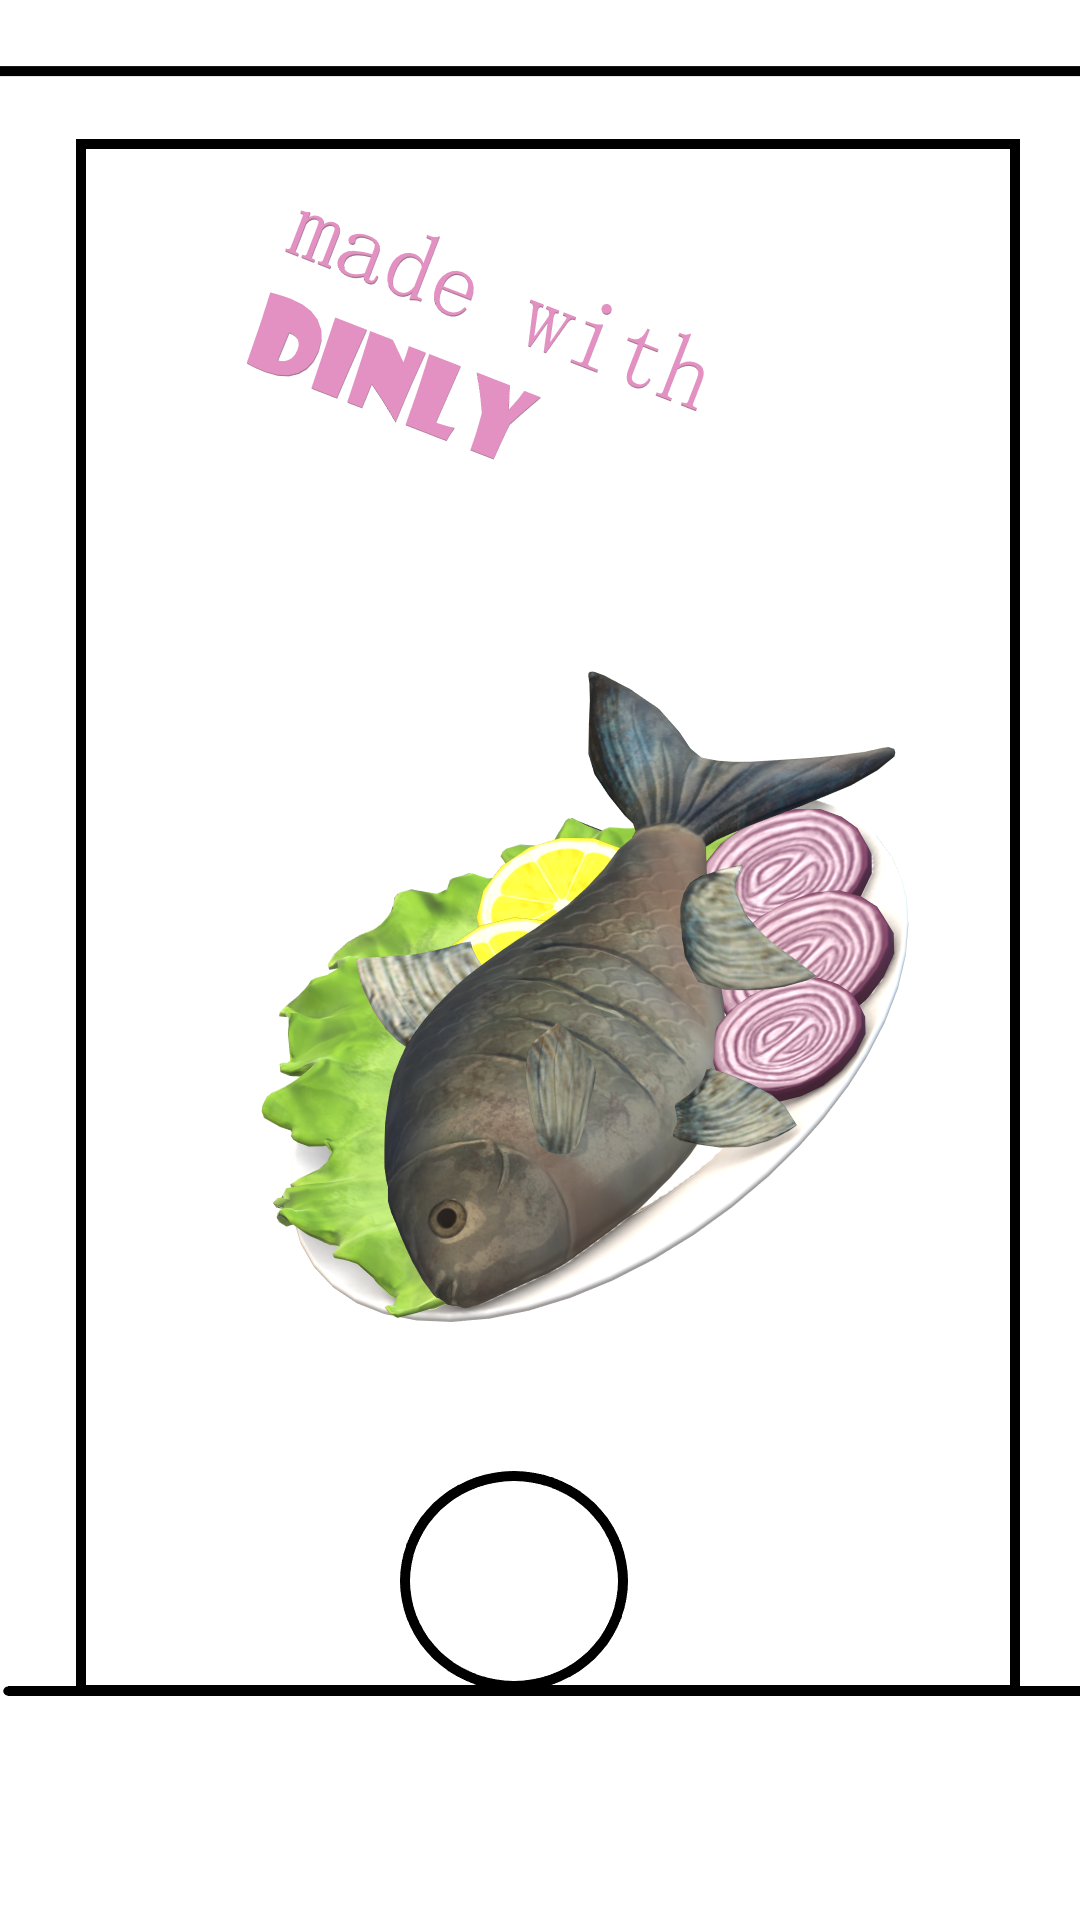
\includegraphics[width=0.4\textwidth]{res/images/Share.png}
\end{center}


\subsubsection{The Standard Use}
Ein Benutzer bereitet eine Mahlzeit zu und bekommt ein Pop-Up, ob er denn ein Foto dieser Mahlzeit teilen möchte. Stimmt der Nutzer zu, so muss er ein Bild aufnehmen und kann dann auswählen auf welcher Platform er dieses Teilen möchte. Daraufhin wird ein Bild mit Wasserzeichen generiert und an die Social Media App weitergereicht.

\subsubsection{The Non-Standard Use}
Der Benutzer bricht während eines Schrittes ab oder verliert seine Internet Verbindung. Sollte er seinen Internetverbindung verlieren muss das Bild gespeichert werden und sobald wieder eine Verbindung besteht wird er gefragt ob er sein Bild nun teilen möchte.
\pagebreak


\section{Non-Functional Requirements}

\subsection{NFR 1: Performance}
\begin{tabular}{|p{.2\linewidth}|p{.65\linewidth}|}
\hline 
ID: & performance \\ \hline
Name: & Performance \\ \hline
Type	: & USE \\ \hline
Descritpion: & Das System muss innerhalb von 300ms antworten  \\ \hline
\end{tabular}

\subsection{NFR 2: Sicherheit}
\begin{tabular}{|p{.2\linewidth}|p{.65\linewidth}|}
\hline 
ID: & security \\ \hline
Name: & Sicherheit \\ \hline
Type	: & SEC \\ \hline
Descritpion: & Die Nutzerdaten dürfen nur verschlüsselt übertragen werden.  \\ \hline
\end{tabular}

\subsection{NFR 3: Porting }
\begin{tabular}{|p{.2\linewidth}|p{.65\linewidth}|}
\hline 
ID: &  porting\\ \hline
Name: & Porting \\ \hline
Type	: & MAINT \\ \hline
Descritpion: & Die App muss auf Andriod und iOS geported werden können.  \\ \hline
\end{tabular}

\subsection{NFR 4: Wartbarkeit }
\begin{tabular}{|p{.2\linewidth}|p{.65\linewidth}|}
\hline 
ID: &  maintainability\\ \hline
Name: & Wartbarkeit \\ \hline
Type	: & MAINT \\ \hline
Descritpion: & Da unser Projekt viele Features benötigt, muss die Software einer einfach erweiterbaren Architektur folgen. Dies soll weitere Implementierungen vereinfachen. \\ \hline
\end{tabular}

\pagebreak

\section{Quantity Structure}
Es ist anzustreben, möglichst viele Rezepte und Zutaten zu speichern, um eine bestmögliche Auswahl an Rezepten/Gerichten anbieten zu können. Hierfür müssen zu allen Zutaten die entsprechenden Nährwerte pro 100g gespeichert werden. Zu den Rezepten müssen Daten wie Name,Zutaten und die Zubereitungsschritte gespeichert werden. Diese Daten werden den Großteil der Datensätze ausmachen. Benutzerdaten bestehen aus Benutzname,Email zusätzlich werden noch ernährungsspezifische Daten erfast wie z.B.: Unverträglichkeiten. Zu Beginn wird es sich um wenige Megabyte an Daten handeln, da wir nicht sofort 10 Tausende Rezepte und deren Zutaten haben werden. Selbiges gilt für die Benutzdaten jedoch werden diese im Vergleich zu den Rezepten weniger ausmachen, da hier pro Benutzer nur wenige Felder gespeichert werden müssen. Das System muss einfach horizontal skalierbar sein um eventuellen Datenmengen von vielen 100gb und mehreren 10 Tausend Anfragen pro Tag gewachsen zu sein.

\pagebreak
\section{System Architecture and Interfaces}

\begin{center}
    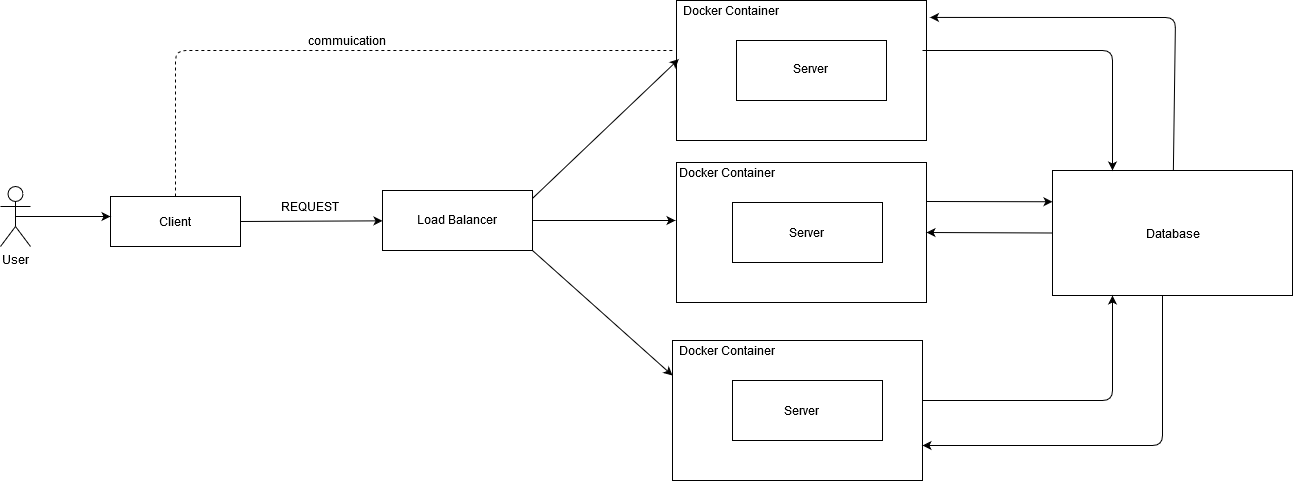
\includegraphics[width=0.9\textwidth]{res/images/System Architecture.png}
\end{center}

\noindent Es braucht sowohl einen Mobile- als auch einen Web- Client, da Rezepte angenehmer per PC hinzugefügt werden können als am Smartphone. Die Server stellen per REST die Rezeptdaten für die Clients zur Verfügung. Sie selbst sind wiederum in Docker- Containern verpackt um vertikales skalieren zu ermöglichen. 

\pagebreak
\section{Acceptance Criteria} 

\subsubsection{Rezeptvorschläge}
\begin{tabular}{|p{.3\linewidth}|p{.7\linewidth}|}
\hline
\cellcolor[gray]{0.5}\textcolor{white}{Steps} & \cellcolor[gray]{0.5}\textcolor{white}{Expected Behavior}\\ \hline
Rezeptvorschläge&Die Rezeptvorschläge müssen zuverlässig sein und den Bedingungen und den Essgewohnheiten des Users entsprechen \\\hline
\end{tabular}

\subsubsection{Rezeptsuche}
\begin{tabular}{|p{.3\linewidth}|p{.7\linewidth}|}
\hline
\cellcolor[gray]{0.5}\textcolor{white}{Steps} & \cellcolor[gray]{0.5}\textcolor{white}{Expected Behavior} \\ \hline
Rezept suchen&Der Nutzer gibt einen Suchtext ein und aktiviert eventuell Filter und bekommt seine gesuchten Rezepte angezeigt. Hierbei werden auch voreingestellt Filter berücksichtigt.\\\hline
Rezept auswählen&Der Nutzer klickt auf ein Rezept und wird auf die Rezeptansicht weitergeleitet.\\\hline
\end{tabular}

\subsubsection{Rezeptdetailansicht}
\begin{tabular}{|p{.3\linewidth}|p{.7\linewidth}|}
\hline
\cellcolor[gray]{0.5}\textcolor{white}{Steps} & \cellcolor[gray]{0.5}\textcolor{white}{Expected Behavior} \\ \hline
Rezept anzeigen&Der Nutzer wählt ein Rezept aus durch die Suche oder durch Vorschläge und erlangt die Detailansicht des Rezepts. Alle Zutaten, Kalorien und die benötigte Kochzeit sind auf dieser Seite aufgelistet.\\\hline
Zutaten zur Einkaufsliste hinzufügen&Der Nutzer wählt alle Zutaten aus die er in die Einkaufsliste hinzufügen möchte. Standardmäßig sind alle Zutaten ausgewählt außer welche die man meistens schon zu Hause hat. Der Nutzer muss nur noch auf einen Button drücken und alle augewählten Zutaten werden auf die Einkaufsliste geschrieben.\\\hline
\end{tabular}

\subsubsection{Rezept erstellen}
\begin{tabular}{|p{.3\linewidth}|p{.7\linewidth}|}
\hline
\cellcolor[gray]{0.5}\textcolor{white}{Steps} & \cellcolor[gray]{0.5}\textcolor{white}{Expected Behavior}\\ \hline
Erstellen & Ein Nutzer kann ein Rezept erstellen, hochladen und für den Eigenbedarf nutzen. \\\hline
Veröffentlichen & Der Nutzer kann sein hochgeladenes Rezept veröffentlichen und so der Allgemeinheit zur Verfügung stellen.\\\hline
\end{tabular}
\subsubsection{Kalorientracker}
\begin{tabular}{|p{.3\linewidth}|p{.7\linewidth}|}
\hline
\cellcolor[gray]{0.5}\textcolor{white}{Steps} & \cellcolor[gray]{0.5}\textcolor{white}{Expected Behavior} \\ \hline
Kalorientracker&Die Erfassung der Gesamtkalorien muss angemessen akkurat erfolgen und eine gute Übersicht über konsumierte Makronährstoffe bieten. \\\hline
\end{tabular}

\subsubsection{Einkaufsliste}
\begin{tabular}{|p{.3\linewidth}|p{.7\linewidth}|}
\hline
\cellcolor[gray]{0.5}\textcolor{white}{Steps} & \cellcolor[gray]{0.5}\textcolor{white}{Expected Behavior} \\ \hline
Einkaufsliste&Das Einfügen und Entfernen eines Artikels muss zuverlässig und schnell erfolgen \\ \hline
Kategorien& Die Artikel werden der richtigen Waren-Kategorie zugeordnet. \\ \hline
Sortieren & Die Kategorien werden richtig sortiert, damit der Einkauf im Supermarkt effizient ist und daher Zeit gespart wird.\\\hline
\end{tabular}



\pagebreak
\end{document}
